% Drawing 154/05-9 -- folder 154, batch 05, archive page 100 (PDF page 101).
% Transcription: page de croquis en couleur, sans texte : deux arbres ramifiés vert clair ; une droite vert clair coupée de droites orange ; un rectangle vert clair partagé en trois bandes verticales (celle du milieu bordée de gris-bleu), traversé d'arcs orange qui délimitent de petits triangles coloriés en orange ; des disques et des demi-disques, bordés de vert clair ou de vert foncé et traversés de pseudo-droites orange, certains avec un arc en tirets gris-bleu ou vert (l'équateur d'un hémisphère vu en perspective) ; une surface allongée, faite d'un disque surmonté et prolongé de deux calottes vert clair, dans laquelle se tressent des courbes orange ; un rectangle aux bords orange traversé de courbes ; un carré vert clair coupé d'une bande en tirets gris-bleu où serpentent des courbes orange
% Kind: page of colour sketches: trees, a striped rectangle, disks and half-disks, an elongated surface. Method 2 (redrawn from the facsimile). Status: ok.
% Notes: Page of colour sketches, no text, redrawn strand by strand from the 400 dpi facsimile (third pass). Trees: two light green vertices, each edge drawn from its computed vertex. Line cut by orange lines: one light green line; the long orange line passes through the crossing of two short ones and through the crossing of the green line with the long oblique (both concurrences exact). Rectangle in three bands: thirteen orange strands traced one by one, each ending on its wall (green side, orange vertical, the dark green or grey-blue border of the middle band); the twelve small orange triangles are filled exactly inside the strands and walls that bound them. Elongated surface: two light green caps above, two light green arcs below, the orange-bordered disk with its grey-blue dashed equator; three orange strands braiding through the upper cap and the disk (one with a small loop), ends on the outer cap and on the disk rim, and an orange diameter. Square: thirteen orange strands, the grey-blue dashed band; one strand bends at its crossing with a horizontal (as drawn), and several strands end on the strand they meet. Disks: the green-rimmed disk at left (six chords and a dashed green diameter), the orange-rimmed disk in the centre (open at the top as on the page; thick orange diameter, six chords, dashed green arc), the disk bottom right (green rim, dark green on its upper half, grey-blue dashed arc, nine strands, three of them through one computed point on the inner orange arc). Half-disk (bowl): dark green rim above, light green below, grey-blue dashed arc, eight orange strands (two pairs through one computed point on the horizontal). Rectangle with orange sides (open at bottom right as on the page): five strands, two of them meeting at a peak above the top side. Lower bowl: light green arc with dashed light green top. In the knot at lower left of the bowl and in the lower half of the square, which stroke continues which is a reading. Redrawn 2026-11-09 (issue 128): to check again. The pairing of the strokes in the two tangles (knot at the lower left of the bowl, lower half of the square) stays a reading: each stroke is followed along its smoothest continuation. Not checked by a reader. Editor's answers (per #153): the reading of the two tangles is accepted as redrawn; the five sets of thin black lines are removed (the three faint pencil strokes beside the trees, the pencil curved triangle left of the centre disk and the vase-shaped pencil outline above the lower bowl; none is in the transcription). 2026-11-14, Claude Opus 5.5, second pass (issue 147): the pencil strokes removed per #153; overlay on the 400 dpi colour scan on a unit grid: every remaining stroke lies on its ink (mean distance under 0.5 unit; none more than 1 unit off over more than a sixth of its length). Not compiled (no TeX in the session). Not checked by a reader.
% Coordinates: 1 unit = 1 mm = 1/100 of the crop width (bbox in page fractions: [0.184, 0.082, 0.837, 0.502]).
% Redrawn by Claude (claude-opus-5-5), issue #73, 2026-11-07; not checked by a human; not compiled (no TeX in the session).
% Redrawn by Claude (claude-opus-5-5) 2026-11-09 (issue #128, third pass): strands traced one by one from the 400 dpi facsimile, crossings computed on the drawn curves, strand ends cut on their rim or wall, concurrent strands through one computed point, coloured triangles filled exactly between their strands; no labels. Status: partial.
% Redrawn stroke by stroke by Claude (claude-opus-5-5) 2026-11-14 (issue #147, second pass): overlaid on the 400 dpi colour facsimile on a unit grid; not compiled (no TeX in the session). Not checked by a human. Status: ok.
% Rights: reproduces part of the work -- behind RENDER_TRANSCRIPTS, never published by itself.
\documentclass[tikz,border=3pt]{standalone}
\usepackage{amsmath,amssymb}
\usetikzlibrary{patterns,arrows.meta}
\tikzset{Or/.style={orange!90!black}, Ye/.style={yellow!80!orange}, Lg/.style={green!60!black!70}, Dg/.style={green!45!black}, Br/.style={brown!80!black}, Rd/.style={red!85!black}, Bl/.style={blue!70!black}, Gy/.style={black!40}, pencil/.style={black!45}, struck/.style={black!35}, mark/.style={circle,draw,inner sep=1.3pt}, pt/.style={circle,fill,inner sep=0.9pt}, opt/.style={circle,draw,fill=white,inner sep=1.1pt}}
\colorlet{Or}{orange!90!black}\colorlet{Ye}{yellow!80!orange}\colorlet{Lg}{green!60!black!70}\colorlet{Dg}{green!45!black}\colorlet{Br}{brown!80!black}\colorlet{Rd}{red!85!black}\colorlet{Bl}{blue!70!black}\colorlet{Gy}{black!40}
\begin{document}
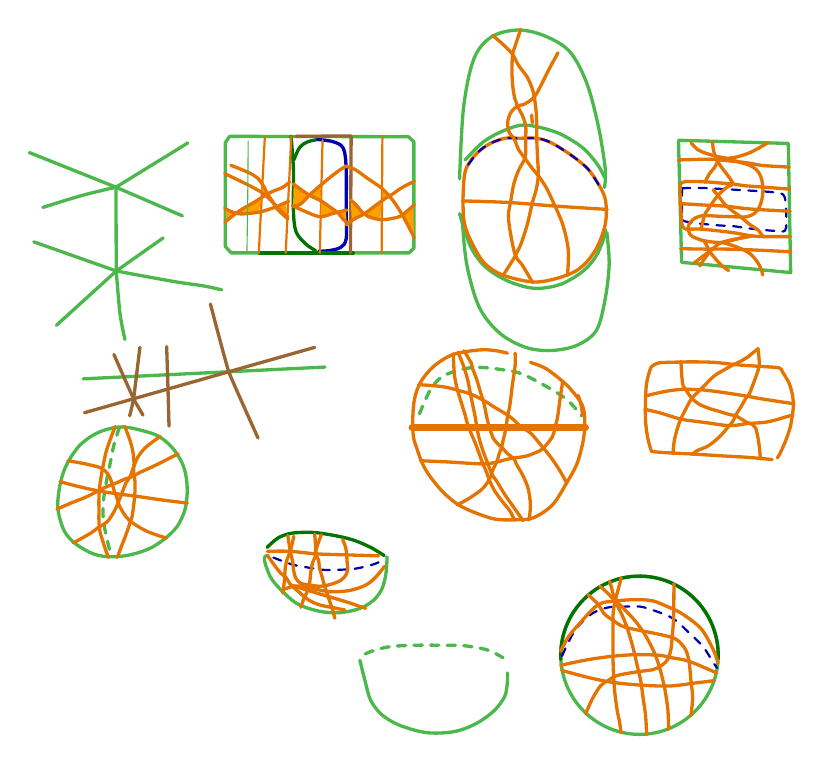
\begin{tikzpicture}[x=1mm,y=1mm,line cap=round,line join=round,font=\scriptsize]
\draw[Lg,very thick] (12.86,-21.06) -- (1.86,-16.66);
\draw[Lg,very thick] (12.86,-21.06) -- (22,-15.43);
\draw[Lg,very thick] (12.86,-21.06) -- (21.3,-24.7);
\draw[Lg,very thick] plot[smooth, tension=0.55] coordinates {(12.86,-21.06) (8.57,-22.1) (3.57,-23.63)};
\draw[Lg,very thick] (12.86,-21.06) -- (12.9,-31.7);
\draw[Lg,very thick] (12.9,-31.7) -- (2.43,-28);
\draw[Lg,very thick] (12.9,-31.7) -- (18.86,-27.5);
\draw[Lg,very thick] (12.9,-31.7) -- (5.3,-38.6);
\draw[Lg,very thick] plot[smooth, tension=0.55] coordinates {(12.9,-31.7) (20,-33) (24,-33.6) (26.3,-34.1)};
\draw[Lg,very thick] plot[smooth, tension=0.55] coordinates {(12.9,-31.7) (13,-33) (13.4,-37.3) (14,-40.4)};
\draw[Lg,very thick] (8.7,-45.4) -- (39.4,-43.9);
\draw[Br,very thick] (8.86,-49.7) -- (38.1,-41.4);
\draw[Br,very thick] plot[smooth, tension=0.2] coordinates {(24.86,-35.9) (27.19,-44.5) (30.9,-52.9)};
\draw[Br,very thick] plot[smooth, tension=0.2] coordinates {(12.6,-42.3) (15.1,-47.93) (16.3,-50)};
\draw[Br,very thick] plot[smooth, tension=0.2] coordinates {(15.9,-41.4) (15.1,-47.93) (14.6,-50.1)};
\draw[Br,very thick] plot[smooth, tension=0.2] coordinates {(19.3,-41.3) (19.45,-46) (19.6,-51.4)};
\draw[Lg,very thick] (26.75,-15.4) -- (27.3,-14.6) -- (50,-14.65) -- (50.7,-15.3) -- (50.7,-28.8) -- (50.1,-29.4) -- (27.5,-29.4) -- (26.75,-28.6) -- (26.75,-15.4);
\draw[Dg,very thick] plot[smooth, tension=0.55] coordinates {(35.1,-14.6) (35.4,-18.8) (35.4,-24.1) (35.75,-26.75) (37,-28.3) (38.2,-29.1)};
\draw[Dg,very thick] plot[smooth, tension=0.55] coordinates {(35.45,-17.6) (36.2,-16) (37.2,-15.3) (38.5,-15)};
\draw[Bl,very thick] plot[smooth, tension=0.55] coordinates {(38.5,-15) (40.5,-15.3) (41.75,-16.15) (42.1,-18.8) (42.1,-24.1) (42.1,-27.6) (41.4,-28.7) (40,-29.1) (38.6,-29.2)};
\draw[Br,very thick] (35.75,-14.6) -- (42.6,-14.55);
\draw[Dg,very thick] (31.1,-29.4) -- (43,-29.4);
\draw[Or,thick] (31.77,-14.6) -- (31,-29.4);
\draw[Or,thick] (35.13,-14.6) -- (34.42,-29.4);
\draw[Or,thick] (39.1,-15.1) -- (38.75,-29.4);
\draw[Br,very thick] (42.73,-14.55) -- (42.64,-29.4);
\draw[Or,thick] (46.7,-14.7) -- (46.6,-29.4);
\fill[orange!75!yellow] (26.75,-23.78) -- (27.06,-23.97) -- (27.38,-24.12) -- (27.74,-24.26) -- (28.07,-24.37) -- (27.77,-24.62) -- (27.49,-24.85) -- (27.21,-25.08) -- (26.92,-25.32) -- cycle;
\fill[orange!75!yellow] (28.09,-24.38) -- (28.45,-24.46) -- (28.82,-24.46) -- (29.2,-24.45) -- (29.57,-24.43) -- (29.92,-24.4) -- (30.3,-24.35) -- (30.65,-24.29) -- (31,-24.22) -- (31.37,-22.36) -- (31.07,-22.56) -- (30.75,-22.77) -- (30.45,-22.95) -- (30.14,-23.13) -- (29.83,-23.3) -- (29.51,-23.47) -- (29.19,-23.66) -- (28.88,-23.84) -- (28.57,-24.03) -- (28.27,-24.24) -- cycle;
\fill[orange!75!yellow] (31.45,-20.66) -- (31.37,-22.36) -- (31.67,-22.18) -- (31.97,-22) -- (31.95,-21.64) -- (31.82,-21.31) -- (31.66,-21) -- (31.47,-20.69) -- cycle;
\fill[orange!75!yellow] (33.14,-23.57) -- (33.48,-23.44) -- (33.8,-23.29) -- (34.13,-23.14) -- (34.47,-23) -- (34.63,-25.04) -- (34.35,-24.79) -- (34.09,-24.56) -- (33.83,-24.31) -- (33.55,-24.08) -- (33.32,-23.81) -- cycle;
\fill[orange!75!yellow] (35.42,-20.68) -- (35.72,-20.92) -- (36.03,-21.15) -- (36.36,-21.38) -- (36.68,-21.6) -- (37.01,-21.82) -- (37.35,-22.03) -- (37.15,-22.35) -- (36.92,-22.63) -- (36.68,-22.9) -- (36.41,-23.12) -- (36.1,-23.32) -- (35.77,-23.46) -- (35.42,-23.51) -- (35.37,-23.13) -- (35.37,-22.72) -- (35.38,-22.33) -- (35.38,-21.97) -- (35.39,-21.61) -- (35.41,-21.24) -- (35.42,-20.85) -- cycle;
\fill[orange!75!yellow] (37.42,-22.07) -- (37.68,-21.83) -- (37.94,-21.59) -- (38.21,-21.35) -- (38.5,-21.11) -- (38.79,-20.87) -- (38.91,-22.81) -- (38.6,-22.63) -- (38.27,-22.48) -- (37.93,-22.35) -- (37.6,-22.17) -- cycle;
\fill[orange!75!yellow] (38.91,-22.81) -- (39.21,-22.99) -- (39.52,-23.19) -- (39.83,-23.41) -- (40.12,-23.63) -- (40.41,-23.84) -- (40.71,-24.04) -- (40.99,-24.24) -- (40.64,-24.33) -- (40.29,-24.43) -- (39.95,-24.57) -- (39.63,-24.72) -- (39.28,-24.8) -- (38.89,-24.81) -- cycle;
\fill[orange!75!yellow] (41,-24.25) -- (41.34,-24.16) -- (41.69,-24.08) -- (42.04,-24) -- (42.1,-24.44) -- (42.11,-24.85) -- (42.12,-25.27) -- (41.78,-25.18) -- (41.54,-24.92) -- (41.33,-24.63) -- (41.1,-24.35) -- cycle;
\fill[orange!75!yellow] (42.68,-22.71) -- (42.97,-22.94) -- (43.24,-23.19) -- (43.5,-23.46) -- (43.73,-23.74) -- (43.95,-24.03) -- (44.2,-24.3) -- (44.08,-24.64) -- (43.75,-24.77) -- (43.42,-24.93) -- (43.11,-25.12) -- (42.81,-25.32) -- cycle;
\fill[orange!75!yellow] (44.36,-24.47) -- (44.64,-24.7) -- (44.99,-24.83) -- (45.34,-24.97) -- (45.67,-25.07) -- (46.03,-25.13) -- (46.41,-25.16) -- (46.65,-22.78) -- (46.35,-22.99) -- (46.05,-23.21) -- (45.76,-23.43) -- (45.47,-23.65) -- (45.19,-23.87) -- (44.91,-24.1) -- (44.61,-24.31) -- cycle;
\fill[orange!75!yellow] (46.66,-21.23) -- (46.93,-21.45) -- (47.18,-21.7) -- (47.42,-21.98) -- (47.32,-22.33) -- (47.02,-22.52) -- (46.73,-22.72) -- cycle;
\fill[orange!75!yellow] (49.23,-24.58) -- (49.53,-24.36) -- (49.82,-24.13) -- (50.1,-23.9) -- (50.37,-23.65) -- (50.64,-23.39) -- (50.7,-27.39) -- (50.54,-27.07) -- (50.37,-26.73) -- (50.2,-26.4) -- (50.04,-26.08) -- (49.87,-25.76) -- (49.71,-25.44) -- (49.53,-25.12) -- (49.35,-24.8) -- cycle;
\draw[Or,very thick] plot[smooth, tension=0.55] coordinates {(27.45,-18.27) (29.6,-19.15) (30.8,-19.86) (31.6,-20.9) (32.04,-21.8) (32.74,-22.86) (33.27,-23.75) (33.98,-24.45) (34.69,-25.09)};
\draw[Or,very thick] plot[smooth, tension=0.55] coordinates {(26.68,-19.34) (28.15,-20.04) (29.9,-20.9) (31.33,-21.7) (32.3,-22.5) (33.3,-23.55) (34,-24.25) (34.7,-24.86)};
\draw[Or,very thick] plot[smooth, tension=0.55] coordinates {(26.69,-25.52) (28,-24.45) (29.03,-23.75) (30.45,-22.95) (31.7,-22.16) (32.74,-21.6) (34,-21.1) (34.91,-20.42)};
\draw[Or,very thick] plot[smooth, tension=0.55] coordinates {(26.68,-23.73) (27.8,-24.28) (29.03,-24.45) (31.15,-24.19) (32.9,-23.66) (34.16,-23.13) (34.81,-22.85)};
\draw[Or,very thick] plot[smooth, tension=0.55] coordinates {(35.35,-20.63) (37.3,-22) (38.9,-22.8) (40.5,-23.9) (41.05,-24.3) (41.7,-25.1) (42.19,-25.54)};
\draw[Or,very thick] plot[smooth, tension=0.55] coordinates {(35.31,-23.41) (36.8,-24.1) (38.75,-24.8) (40.5,-24.37) (41.6,-24.1) (42.18,-23.97)};
\draw[Or,very thick] plot[smooth, tension=0.55] coordinates {(35.3,-23.49) (36.3,-23.2) (37.5,-22) (38.75,-20.9) (40.2,-19.7) (41.4,-18.8) (42.15,-18.36)};
\draw[Or,very thick] plot[smooth, tension=0.55] coordinates {(42.01,-18.4) (43.2,-18.8) (44.9,-20) (46.5,-21.1) (47.6,-22.2) (48.5,-23.4) (49.35,-24.8) (50.2,-26.4) (50.74,-27.47)};
\draw[Or,very thick] plot[smooth, tension=0.55] coordinates {(42.08,-25.86) (43.3,-25) (44.4,-24.45) (45.8,-23.4) (47.05,-22.5) (47.9,-22) (49.2,-21.1) (50.77,-20.31)};
\draw[Or,very thick] plot[smooth, tension=0.55] coordinates {(42.62,-22.67) (43.35,-23.3) (44.2,-24.3) (44.9,-24.8) (46.5,-25.17) (48.1,-25) (49.2,-24.6) (50.76,-23.27)};
\draw[Lg] plot[smooth, tension=0.55] coordinates {(29.65,-15.2) (29.6,-22) (29.5,-29.1)};
\draw[Lg,very thick] plot[smooth, tension=0.55] coordinates {(56.5,-20) (57,-11) (58.3,-4.8) (60.5,-2) (63.8,-1.1) (67.1,-1.76) (70.4,-3.74) (72.6,-7.7) (74.1,-13.2) (75,-18.7) (74.9,-21.1)};
\draw[Lg,very thick] plot[smooth, tension=0.55] coordinates {(57.2,-17.6) (59.4,-15.4) (61.6,-14.1) (64.2,-13.2) (66.4,-13.4) (69.3,-14.3) (72.2,-16.1) (74.1,-18.3) (74.9,-19.8)};
\draw[Lg,very thick] plot[smooth, tension=0.55] coordinates {(56.5,-24.4) (57.9,-28.6) (59.8,-31.2) (62.7,-33) (66,-33.9) (69.3,-33.4) (72.2,-31.7) (73.9,-29.7) (74.9,-27.3) (75,-26.4)};
\draw[Lg,very thick] plot[smooth, tension=0.55] coordinates {(56.8,-24.6) (57.4,-30.8) (59,-36.3) (61.6,-39.6) (64.9,-41.4) (68.2,-41.8) (71.5,-41.1) (73.9,-39.2) (75,-35.2) (75.5,-30.8) (75.2,-26.8)};
\draw[Or,very thick] plot[smooth cycle, tension=0.55] coordinates {(56.94,-22.8) (57.15,-25.8) (58.2,-28.4) (59.7,-30.75) (62.1,-32.26) (66.2,-33.1) (70.05,-32.26) (72.2,-31) (73.9,-28.8) (75,-25.8) (75.1,-23.2) (74.6,-21.5) (73.1,-19.1) (71.8,-17.85) (70.05,-16.56) (67.9,-15.3) (66.2,-14.84) (64,-14.84) (62.3,-14.84) (60.4,-15.5) (58.9,-16.56) (57.8,-17.85) (57.15,-19.35)};
\draw[Bl,dashed,thick] plot[smooth, tension=0.55] coordinates {(57.6,-18.2) (58.9,-16.56) (60.4,-15.5) (62.3,-14.84) (64,-14.84) (66.2,-14.84) (67.9,-15.3) (70.05,-16.56) (71.8,-17.85) (73.1,-19.1) (74.6,-21.5)};
\draw[Or,very thick] plot[smooth, tension=0.55] coordinates {(60.7,-1.78) (62.1,-3) (63.24,-4.2) (64,-5.6) (65.1,-7.1) (65.75,-8.6) (66,-9.7) (66.2,-11.2) (66.3,-12.9) (66.3,-14.84) (66.4,-17.2) (66.5,-19.6) (66.2,-21.5) (65.75,-23) (65.1,-25.8) (64.25,-28.4) (63.6,-29.75) (62,-32.31)};
\draw[Or,very thick] plot[smooth, tension=0.55] coordinates {(64.26,-1.01) (63.6,-3) (63.24,-4.2) (63.15,-6.45) (63.3,-8.6) (63.55,-9.9) (63.85,-10.75) (64.5,-12) (64.9,-13.3) (64.9,-14.84) (64.9,-16.3) (64.8,-17.4) (64,-18.9) (63.4,-20.6) (63,-22.8) (62.7,-24.7) (63,-27.1) (63.6,-29.75) (64.5,-31) (65.77,-33.17)};
\draw[Or,very thick] plot[smooth, tension=0.55] coordinates {(69,-4) (67.9,-6) (66.8,-8.2) (66,-9.6) (65.1,-10.3) (64.5,-10.6) (63.85,-10.75) (63,-11.6) (62.6,-12.9) (62.85,-14.2) (63.4,-14.84) (64,-16.3) (64.8,-17.4) (65.75,-18.7) (66.5,-19.6) (67.5,-21.1) (68.5,-23.2) (69.6,-25.8) (70.3,-29) (70.2,-32.29)};
\draw[Or,very thick] plot[smooth, tension=0.55] coordinates {(56.86,-22.8) (62.74,-23) (68.55,-23.45) (75.25,-23.88)};
\draw[Or,very thick] (65.65,-11.9) -- (65.75,-12.9);
\draw[Lg,very thick] (84.3,-15.1) -- (98.25,-15.5) -- (98.55,-31.9) -- (84.7,-30.6) -- (84.3,-15.1);
\draw[Bl,dashed,thick] plot[smooth, tension=0.55] coordinates {(84.75,-21.2) (87.1,-21.15) (91.8,-21.4) (96.4,-21.7) (97.6,-22) (97.9,-23) (98,-25.5) (97.8,-26.6) (96.4,-26.6) (93.3,-26.3) (91.2,-26) (89.3,-25.9) (85.6,-25.5) (84.85,-25) (84.75,-23) (84.75,-21.2)};
\draw[Or,very thick] plot[smooth, tension=0.55] coordinates {(84.28,-17.6) (86,-17.55) (88.4,-17.5) (89.5,-17.6) (91.6,-17.8) (93.3,-18) (95,-18.3) (98.38,-18.51)};
\draw[Or,very thick] plot[smooth, tension=0.55] coordinates {(85.9,-15.43) (86.8,-16.33) (87.94,-16.8) (89.1,-17.13) (90.4,-17.4) (92.1,-17.9) (93.3,-18.26) (94.2,-18.83) (94.75,-19.7) (95,-20.87) (95,-22) (94.75,-23.14) (94.3,-24.04) (93.6,-24.6) (92.7,-24.84) (91.9,-24.84) (89.5,-24.75) (87.5,-24.67) (86.47,-24.95) (85.8,-25.5) (85.56,-26.1) (85.67,-26.88) (86.1,-27.33) (87.26,-27.79) (88.4,-28) (89.87,-28.1) (90.4,-27.98) (92.1,-27.56) (93.74,-27.23)};
\draw[Or,very thick] plot[smooth, tension=0.4] coordinates {(98.44,-21.31) (95,-21.04) (92.7,-20.87) (91.2,-20.65) (90.4,-20.6) (89.3,-20.5) (87.5,-20.36) (85.2,-20.35) (84.6,-20.6) (84.5,-21.6) (84.6,-24) (84.75,-25.8) (85.2,-26.37) (87.04,-26.37) (89.3,-26.6) (91.57,-26.88) (93.3,-27.2) (95,-27.33) (98.55,-27.33)};
\draw[Or,very thick] plot[smooth, tension=0.55] coordinates {(84.5,-23.14) (88.17,-23.36) (90.4,-23.48) (92.7,-23.76) (95,-23.93) (98.49,-24.11)};
\draw[Or,very thick] plot[smooth, tension=0.55] coordinates {(84.58,-28.87) (87.6,-28.92) (90.4,-28.92) (93.84,-29.03) (98.58,-29.26)};
\draw[Or,very thick] plot[smooth, tension=0.55] coordinates {(95.65,-15.4) (95,-15.8) (93.3,-16.7) (91.6,-17.24) (90.9,-17.35) (89.5,-17.6) (88.85,-18.6) (88.2,-19.4) (87.67,-20.44)};
\draw[Or,very thick] plot[smooth, tension=0.45] coordinates {(88.62,-15.26) (88.75,-16.4) (89.1,-17.4) (89.6,-18.3) (90.2,-19.1) (90.8,-19.9) (91.2,-20.65) (90.4,-21.1) (89.5,-21.9) (88.85,-22.7) (88.17,-23.7) (87.7,-24.4) (87.4,-25.4) (87.17,-26.46)};
\draw[Or,very thick] plot[smooth, tension=0.55] coordinates {(88.7,-21.4) (89.4,-22.2) (90.2,-23.25) (91.2,-24.1) (92.1,-24.75) (93.3,-25.75) (94.4,-26.5) (95.07,-27.39)};
\draw[Or,very thick] plot[smooth, tension=0.55] coordinates {(87.49,-27.8) (87.83,-28.35) (88.28,-29.26) (88.8,-29.9) (89.3,-30.5) (89.87,-31.07) (90.66,-31.64)};
\draw[Or,very thick] plot[smooth, tension=0.55] coordinates {(87,-31.07) (87.5,-30.3) (88.28,-29.26) (88.9,-28.65) (89.6,-28.15) (90.6,-27.85) (92.1,-27.52) (93.69,-27.23)};
\draw[Or,very thick] plot[smooth, tension=0.55] coordinates {(86.24,-30.73) (87.3,-29.9) (88.32,-29.17)};
\draw[Or,very thick] plot[smooth, tension=0.55] coordinates {(89.92,-28.08) (91.57,-28.6) (93.04,-29.26) (93.84,-29.94) (94.5,-30.85) (94.86,-31.64) (95,-32.2)};
\draw[Lg,very thick] plot[smooth cycle, tension=0.55] coordinates {(13.67,-51.5) (16.1,-51.94) (18.3,-52.7) (20.06,-54.2) (21.27,-56.1) (21.8,-58) (21.9,-60.05) (21.6,-62.1) (20.6,-64.2) (19,-65.75) (17.1,-66.96) (14.7,-67.74) (12.3,-68) (10.05,-67.65) (7.8,-66.4) (6.4,-64.9) (5.64,-62.8) (5.47,-61.1) (5.73,-59) (6.25,-57.1) (7.1,-55.4) (8.3,-53.8) (9.87,-52.6) (11.6,-51.85)};
\draw[Lg,dashed,very thick] plot[smooth, tension=0.55] coordinates {(13.3,-51.55) (12.6,-53.8) (12.1,-56.25) (11.6,-58.7) (11.25,-61.1) (11.25,-63.2) (11.6,-65.2) (12.1,-67.3) (12.3,-68)};
\draw[Or,very thick] plot[smooth, tension=0.55] coordinates {(12.75,-51.45) (12.1,-53.2) (11.6,-54.7) (11.2,-56.6) (10.97,-57.87) (10.78,-59.13) (10.7,-60.4) (10.7,-62.3) (10.7,-63.57) (10.84,-64.83) (11.22,-66.1) (11.88,-68.07)};
\draw[Or,very thick] plot[smooth, tension=0.55] coordinates {(13.97,-51.43) (14.64,-53.2) (15.02,-54.7) (15.15,-56.1) (15.1,-57.1) (15.27,-58.37) (15.27,-59.77) (15.15,-61.16) (14.9,-62.93) (14.64,-63.7) (14.13,-65.2) (13.63,-66.48) (13.03,-68.08)};
\draw[Or,very thick] plot[smooth, tension=0.55] coordinates {(18.48,-52.72) (16.67,-54.07) (15.65,-55.33) (15.1,-56.6) (14.64,-57.87) (14.13,-58.63) (13.63,-59.9) (13.12,-61.16) (12.6,-62.3) (11.73,-63.57) (10.7,-64.2) (9.7,-64.96) (7.46,-66.24)};
\draw[Or,very thick] plot[smooth, tension=0.55] coordinates {(20.76,-54.92) (17.93,-56.35) (16.03,-57.23) (14.77,-57.87) (14,-58.12) (12.87,-58.63) (11.6,-59.13) (10.59,-59.64) (9.07,-60.4) (7.17,-61.16) (5.37,-61.95)};
\draw[Or,very thick] plot[smooth, tension=0.55] coordinates {(6.77,-55.79) (9.07,-56.22) (10.97,-56.73) (11.85,-57.5) (12.36,-58.63) (12.6,-59.5) (12.95,-60.4) (13.37,-61.67) (14.5,-63.3) (16.67,-64.7) (19.27,-65.63)};
\draw[Or,very thick] plot[smooth, tension=0.55] coordinates {(5.75,-58.45) (8,-59.05) (10.5,-59.6) (13,-60) (15.4,-60.3) (18.5,-60.75) (21.93,-61.18)};
\draw[Or,very thick] plot[smooth, tension=0.55] coordinates {(65.5,-43.3) (67.47,-44.1) (69.6,-45.73) (70.74,-46.87) (72.05,-48.67) (72.4,-50.6) (72.2,-53.25) (71.4,-56.2) (70.1,-58.6) (68.3,-61.4) (65.84,-63.05) (63.4,-63.3) (60.94,-63.2) (58.5,-62.4) (56.36,-61.4) (54.4,-59.78) (52.77,-57.82) (51.8,-56.2) (51.13,-54.4) (50.64,-52.75) (50.56,-50.3) (50.8,-47.85) (51.6,-45.73) (53.26,-43.77) (55.7,-42.3) (58.98,-41.73) (60.94,-41.8) (62.57,-42.13)};
\draw[Lg,dashed,very thick] plot[smooth, tension=0.55] coordinates {(51.4,-49.85) (52.84,-46.7) (54.6,-44.95) (58.2,-43.95) (62.4,-44.3) (64.6,-44.85) (67.76,-46.5) (70.2,-48.1) (72,-50.1)};
\draw[Or,very thick] plot[smooth, tension=0.55] coordinates {(71.56,-47.5) (71.9,-48.6) (72.13,-49.98)};
\draw[Or,line width=2.4pt] plot[smooth, tension=0.55] coordinates {(50.44,-51.6) (61,-51.6) (72.51,-51.6)};
\draw[Or,very thick] plot[smooth, tension=0.55] coordinates {(55.7,-42.22) (55.8,-44.4) (55.87,-45.1) (56.2,-46.7) (56.7,-48.35) (57.2,-49.98) (57.5,-51.1) (58,-52.4) (58.5,-53.57) (58.98,-54.88) (59.47,-56.2) (59.96,-57.33) (60.3,-58.3) (60.94,-59.6) (61.9,-60.93) (62.9,-62.2) (63.49,-63.37)};
\draw[Or,very thick] plot[smooth, tension=0.55] coordinates {(56.31,-42.01) (57,-43.77) (57.5,-45.4) (57.83,-47.04) (58.16,-48.67) (58.5,-50.3) (58.7,-51.6) (58.98,-52.92) (59.47,-54.55) (60.1,-56.2) (60.6,-57.5) (61.26,-58.47) (62.25,-60.1) (63.4,-61.74) (64.57,-63.42)};
\draw[Or,very thick] plot[smooth, tension=0.55] coordinates {(57.08,-41.83) (58,-43.44) (58.16,-44.1) (58.65,-45.4) (59.14,-47.04) (59.63,-48.67) (59.96,-50.3) (60.3,-51.6) (60.77,-52.92) (61.3,-53.6) (61.84,-54.06) (62.57,-54.88) (63.4,-55.53) (63.7,-56.2) (64.53,-57.66) (65.2,-59.3) (65.5,-61.4) (65.33,-63.31)};
\draw[Or,very thick] plot[smooth, tension=0.55] coordinates {(63.55,-42.13) (63.55,-43.77) (63.2,-46.2) (62.9,-48.67) (62.57,-50.3) (62.4,-51.6) (62.1,-52.92) (61.84,-54.06) (61.5,-55) (61.26,-55.86) (60.77,-56.84) (60.45,-57.8) (60.1,-58.47) (59.3,-59.45) (57.67,-60.6) (56.22,-61.4)};
\draw[Or,very thick] plot[smooth, tension=0.55] coordinates {(51.53,-55.8) (55,-55.95) (59.3,-56.2) (60.94,-56.03) (62.57,-55.6) (63.4,-55.45) (65,-55.2) (66.66,-54.55) (67.15,-54.2) (68.3,-52.75) (68.6,-51.6) (68.94,-50.3) (69.27,-47.85) (69.61,-45.65)};
\draw[Or,very thick] plot[smooth, tension=0.55] coordinates {(51.28,-46.13) (54.4,-46.4) (56.36,-46.87) (58,-47.36) (59.63,-48.18) (60.94,-49) (62.57,-49.98) (63.4,-50.63) (64.2,-51.4) (65.5,-52.27) (66.5,-53.4) (67.15,-54.2) (67.97,-55.2) (69.1,-56.84) (70.14,-58.67)};
\draw[Or,very thick] plot[smooth, tension=0.45] coordinates {(96.2,-55.64) (93,-55.36) (90.2,-55.2) (86,-54.94) (83.2,-54.8) (81.1,-54.65) (80.82,-54.45) (80.4,-52.9) (80.12,-50.8) (80.12,-48) (80.26,-45.9) (80.82,-43.94) (81.8,-43.38) (83.2,-43.3) (86,-43.24) (88.8,-43.3) (90.9,-43.52) (92.3,-43.66) (94.4,-43.8) (97.07,-44) (97.5,-44.5) (98.33,-45.9) (98.75,-47.3) (98.9,-48.7) (98.75,-50.1) (98.47,-51.64) (97.9,-53.3) (97.2,-54.87) (96.86,-55.43)};
\draw[Or,very thick] plot[smooth, tension=0.55] coordinates {(83.6,-54.9) (83.76,-53.3) (84.18,-51.64) (84.6,-50.5) (85.3,-49.1) (86,-47.86) (87.26,-46.6) (88.8,-45.06) (90.2,-44.2) (90.9,-43.8) (92.3,-43.1) (93,-42.7) (94.4,-41.56)};
\draw[Or,very thick] plot[smooth, tension=0.55] coordinates {(94.4,-41.56) (94.48,-42.26) (94.55,-43.8) (94.1,-45.2) (93.3,-47.3) (92.86,-47.86) (92.3,-48.84) (91.6,-49.96) (91.2,-50.8) (90.5,-51.64) (89.5,-52.76) (88.1,-53.9) (86.7,-54.5) (86.05,-54.99)};
\draw[Or,very thick] plot[smooth, tension=0.55] coordinates {(84.61,-43.18) (84.74,-45.2) (84.9,-46.3) (85.3,-46.9) (86,-47.86) (86.84,-48.56) (88.1,-49.12) (89.5,-49.54) (90.9,-49.96) (91.6,-50.1) (92.3,-50.52) (93,-50.94) (93.7,-51.2) (94.1,-51.64) (94.4,-52.9) (94.6,-54.3) (94.7,-55.58)};
\draw[Or,very thick] plot[smooth, tension=0.55] coordinates {(80.05,-47.58) (81.8,-47.16) (83.2,-46.9) (84.6,-46.74) (86,-46.74) (87.4,-46.8) (90.2,-47.16) (93,-47.6) (94.4,-47.86) (97.2,-48.3) (98.98,-48.56)};
\draw[Or,very thick] plot[smooth, tension=0.55] coordinates {(80.01,-49.26) (81.8,-49.68) (83.2,-50.1) (84.6,-50.52) (86,-50.73) (88.1,-51) (90.2,-51.3) (91.6,-51.3) (93,-51.08) (95.1,-50.94) (96.5,-50.66) (97.9,-50.24) (98.84,-49.99)};
\draw[Dg,very thick] plot[smooth, tension=0.55] coordinates {(32.07,-66.8) (33.45,-65.6) (35.2,-65) (37.8,-64.9) (40.36,-65.25) (42.95,-65.85) (45.2,-66.8) (46.93,-67.84)};
\draw[Lg,very thick] plot[smooth, tension=0.55] coordinates {(31.9,-67.84) (31.73,-68.53) (32.6,-70.77) (34.3,-72.67) (36.05,-74.05) (38.64,-74.9) (41.2,-75.1) (43.8,-74.57) (45.55,-73.53) (46.6,-72.15) (47.1,-70.43) (47.27,-68.7) (47.27,-68)};
\draw[Bl,dashed,thick] plot[smooth, tension=0.55] coordinates {(32.85,-68.1) (35.2,-68.96) (36.9,-69.3) (39.15,-69.65) (41.05,-69.65) (43.3,-69.5) (45.55,-68.96) (46.6,-68.5)};
\draw[Or,very thick] plot[smooth, tension=0.55] coordinates {(32.1,-67.3) (35,-67.3) (38.23,-67.62) (42.03,-67.75) (46.2,-67.88)};
\draw[Or,very thick] plot[smooth, tension=0.55] coordinates {(35.45,-65.4) (35,-67.3) (34.6,-68.3) (34.35,-69.5) (34.3,-70.5) (34.2,-71.5) (34.05,-72.6)};
\draw[Or,very thick] plot[smooth, tension=0.55] coordinates {(34.69,-65.3) (35,-67.3) (35.32,-68.7) (35.4,-69.6) (35.7,-70.7) (36.33,-71.36) (37.6,-71.6) (38.87,-71.74) (40.13,-71.5) (41.4,-71) (42.03,-70.35) (42.29,-69.6) (42.22,-68.7) (42.16,-67.7) (42.03,-66.8) (41.65,-65.8)};
\draw[Or,very thick] plot[smooth, tension=0.55] coordinates {(38.1,-65.1) (38.23,-67.62) (37.85,-68.7) (37.6,-69.97) (37.47,-71.23) (37.1,-72.5) (36.7,-73.39) (36.33,-74.4)};
\draw[Or,very thick] plot[smooth, tension=0.55] coordinates {(38.93,-65.2) (38.36,-66.8) (38.23,-67.62) (38.6,-68.45) (38.7,-69.4) (39,-70.4) (39.37,-71.74) (39.75,-72.88) (40.13,-74) (40.5,-75.16) (40.64,-75.8)};
\draw[Or,very thick] plot[smooth, tension=0.55] coordinates {(46.97,-69.2) (45.83,-70.6) (44.57,-71.6) (42.67,-72.25) (40.77,-72.44) (39.5,-72.37) (38.2,-72.1) (36.8,-71.8) (35.6,-71.7) (34.04,-72.17)};
\draw[Or,very thick] plot[smooth, tension=0.55] coordinates {(32.1,-67.8) (32.9,-68.95) (33.8,-70.1) (34.43,-70.6) (35.07,-71.6) (35.7,-72.12) (36.7,-73) (37.6,-73.64) (38.87,-74.15) (40.13,-74.4) (41.4,-74.65) (41.9,-74.72)};
\draw[Or,very thick] plot[smooth, tension=0.55] coordinates {(34.99,-71.57) (37.6,-72.37) (38.87,-72.75) (40.13,-73.13) (41.4,-73.5) (42.67,-73.9) (43.93,-74.34) (44.57,-74.53)};
\draw[Lg,very thick] plot[smooth, tension=0.55] coordinates {(43.84,-81.14) (44.53,-83.9) (45.2,-86.2) (46.6,-88.03) (48.9,-89.4) (52.34,-90.33) (55.8,-90.2) (58.55,-89.2) (60.85,-87.57) (62.23,-85.74) (62.57,-83.9) (62.57,-82.75)};
\draw[Lg,dashed,very thick] plot[smooth, tension=0.55] coordinates {(44.53,-80.33) (45.68,-79.87) (47.75,-79.4) (50.85,-79.23) (54.2,-79.23) (57.17,-79.3) (60.16,-79.87) (62.34,-81.02)};
\draw[Lg,very thick] (79.35,-80.5) ellipse[x radius=10, y radius=10.05];
\draw[Dg,very thick] (69.36,-81.03) arc[start angle=183, end angle=-3, x radius=10, y radius=10.05];
\draw[Bl,dashed,thick] plot[smooth, tension=0.55] coordinates {(69.5,-80.6) (71.14,-77.37) (73.23,-75.28) (75.3,-74.44) (77.4,-74.33) (79.5,-74.33) (81.6,-74.96) (83.7,-75.9) (85.8,-77.8) (87.46,-79.46) (88.7,-81.4) (89.2,-82.1)};
\draw[Or,very thick] plot[smooth, tension=0.55] coordinates {(69.33,-80) (70.3,-78.2) (71.83,-76.36) (74.13,-74.06) (76.43,-73.6) (78.74,-73.45) (81.04,-73.6) (83.34,-74.52) (84.87,-75.3) (87.17,-77.13) (88.7,-79.74) (89.33,-81.51)};
\draw[Or,very thick] plot[smooth, tension=0.55] coordinates {(69.35,-81.77) (72.6,-81.1) (75.67,-80.66) (78.74,-80.43) (81.8,-80.5) (83.34,-80.8) (85.64,-81.27) (89.17,-82.76)};
\draw[Or,very thick] plot[smooth, tension=0.55] coordinates {(69.46,-82.42) (72.6,-83.26) (75.05,-83.8) (77.2,-84.1) (80.27,-84.34) (83.34,-84.4) (86.4,-84.03) (88.9,-83.72)};
\draw[Or,very thick] plot[smooth, tension=0.55] coordinates {(72.51,-87.93) (73.37,-86.02) (74.44,-84.34) (75.36,-83.72) (76.43,-83.1) (78.74,-82.65) (81.04,-82.34) (81.8,-82.04) (82.88,-81.12) (83.34,-79.74) (83.5,-78.2) (83.65,-76.36) (83.7,-74.5) (83.73,-71.38)};
\draw[Or,very thick] plot[smooth, tension=0.55] coordinates {(77.04,-70.65) (76.6,-72.3) (76.25,-73.62) (76.1,-74.4) (75.98,-75.5) (75.98,-76.67) (75.98,-80.5) (76.05,-82.8) (76.2,-85.1) (76.5,-87.4) (76.8,-88.9) (77.02,-90.35)};
\draw[Or,very thick] plot[smooth, tension=0.55] coordinates {(75.57,-71.11) (75.9,-72.3) (76.25,-73.62) (76.82,-74.75) (77.36,-75.9) (77.97,-77.6) (78.58,-79.74) (79.04,-81.73) (79.5,-83.72) (79.8,-85.87) (80.12,-88.17) (80.26,-90.59)};
\draw[Or,very thick] plot[smooth, tension=0.55] coordinates {(74.32,-71.73) (75.4,-72.7) (76.25,-73.62) (77,-74.2) (77.5,-74.75) (78.74,-76.06) (79.96,-77.74) (81.04,-79.74) (81.65,-81.27) (82.1,-82.8) (82.57,-84.8) (82.95,-87.4) (83.06,-89.91)};
\draw[Or,very thick] plot[smooth, tension=0.55] coordinates {(72.8,-72.8) (74.13,-74.06) (74.83,-75.2) (75.98,-76.06) (77.2,-76.82) (79.04,-77.28) (81.04,-77.67) (83.34,-78.2) (84.26,-78.66) (85.18,-79.74) (85.64,-81.27) (85.87,-83.57) (86.1,-85.87) (85.88,-88.18)};
\end{tikzpicture}
\end{document}
